% Created 2015-02-26 Thu 10:35
\documentclass[12pt, a4paper]{article}
\usepackage[utf8]{inputenc}
\usepackage[T1]{fontenc}
\usepackage{fixltx2e}
\usepackage{graphicx}
\usepackage{longtable}
\usepackage{float}
\usepackage{wrapfig}
\usepackage{rotating}
\usepackage[normalem]{ulem}
\usepackage{amsmath}
\usepackage{textcomp}
\usepackage{marvosym}
\usepackage{wasysym}
\usepackage{amssymb}
\usepackage{hyperref}
\tolerance=1000
\usepackage{fullpage}
\usepackage{graphicx}
\usepackage{authblk}
\usepackage{mathtools}
\usepackage{setspace} % for adjusting TOC line spacing
\usepackage{algorithm} % typesetting algorithms
\usepackage{algpseudocode} % typesetting algorithms
\renewcommand{\algorithmicrequire}{\textbf{Input:}}
\setlength{\parindent}{0pt}
\setlength{\parskip}{1em}
\setlength{\affilsep}{0.5em}
\usepackage[backend=bibtex,sorting=none]{biblatex}
\usepackage{hyperref}
\addbibresource{refs_supplement.bib}
\author[1]{Aleksandra Vancevska}
\author[1]{Verena Pfeiffer}
\author[2]{Kyle M. Douglass}
\author[1]{Joachim Lingner}
\author[2]{Suliana Manley}
\affil[1]{Swiss Institute for Experimental Cancer Research (ISREC), EPFL, Lausanne, Switzerland}
\affil[2]{Institute of Physics of Biological Systems, EPFL, Lausanne, Switzerland}
\date{}
\title{Supplementary Material}
\hypersetup{
  pdfkeywords={},
  pdfsubject={},
  pdfcreator={Emacs 24.4.50.1 (Org mode 8.2.6)}}
\begin{document}

\maketitle
\setcounter{tocdepth}{2}
\tableofcontents

\begin{abstract}
This is the supplementary material accompanying the manuscript.
\end{abstract}

\section{Telomere size determination from STORM data}
\label{sec-1}

\subsection{Data acquisition}
\label{sec-1-1}
Fixed Hela cells containing Cy5-labeled telomeric DNA were imaged
on an inverted Nikon N-STORM microscope with a 100x/1.49 N.A. Nikon
APO TIRF objective and an Andor iXon3 897 EMCCD camera. Two lasers,
a 500 mW, 640 nm Coherent Sapphire and 100 mW, 402 nm Coherent
Sapphire were used to induce fluorophore switching and to control
the switching rate, respectively. A cylindrical lens was inserted
between the tube lens and camera to introduce a slight astigmatism
to the microscope's point spread function (PSF). The axial
coordinate of all recorded fluorophore localizations was inferred
from the shape of the astigmatic PSF after a calibration routine
\cite{huang-science-2008}.

For imaging, the camera sensor was cropped to $256 \times 256 \;
   \text{pixels}^2$, corresponding to a $40.96 \times 40.96 \; \mu
   m^2$ field of view (FOV) with a square pixel width equivalent to
$0.16 \, \mu m$ in the sample plane. 10,000 images were recorded
for each FOV. Between 10 and 30 FOV's were recorded for each
experiment. The optimal focal plane position for each FOV was
judged by eye as having the greatest number of in-focus
telomeres. Molecule localization and drift correction was performed
in the Nikon NIS-Elements software, version 4.30.01.

The output of the data acquistion stage of an imaging experiment
consisted of lists of detected molecules with their corresponding
drift-corrected x-, y-, and z-positions. A molecule's measured
position combined with the corresponding precision makes one
localization.

\subsection{Clustering and filtering}
\label{sec-1-2}

\subsubsection{Temporal grouping}
\label{sec-1-2-1}
Fluorescent molecules whose centers appeared in the same pixel for
up to 10 consecutive frames were grouped together as one single
localization \cite{annibale-natmethods-2011}. Fluorescent
molecules that appeared in the same pixel for longer than 10
consecutive frames were removed from the analysis since they could
have likely been from dust or other impurities. This step has the
effects of improving localization precisions of single emitters
that emit for a few camera frames and removing spurious noise
localizations.

\subsubsection{Clustering localizations}
\label{sec-1-2-2}
Localizations in each FOV were sorted into clusters corresponding
to individual telomeres using a Matlab implementation of the
density-based spatial clustering of applications with noise
(DBSCAN) algorithm
\cite{daszykowski-chemometrintelllab-2001}. This algorithm was
applied for two reasons. The first was to group localizations
belonging to different telomeres into distinct clusters. The
second reason was to remove localizations not originating from a
telomere from the dataset.

Briefly, the DBSCAN algorithm first randomly selects a
localization in the dataset and determines whether it has a
minimum number of neighboring localizations, $k$, within a sphere
of radius $\epsilon$ surrounding it. This sphere is called the
``neighborhood'' of the localization. If less than $k$
localizations are identified within the neighborhood, the
localization is labeled as noise and a new point is chosen for
processing.

If, on the other hand, there is a sufficient number of other
localizations within the current localization's neighborhood, then
a new cluster is started from this point. The current localization
and all points in its neighborhood are added to the cluster. Then,
the localizations within the neighborhoods of the other points of
the cluster are added if they contain at least $k$
localizations. This process is repeated until all localizations
that are within the cluster are identified. Note that
localizations that may have been identified as noise during
previous iterations of the algorithm can be grouped into a
cluster. These localizations are located at the outer regions of
individual clusters.

The optimum values for the input parameters to the DBSCAN
algorithm are those that group all localizations from individual
telomeres into separate clusters and that also identify
localizations not belonging to telomeres as noise.

To find the optimum values for the input parameters $k$ and
$\epsilon$, a parameter sweep was performed on the STORM data from
the untransfected Hela L and Hela S experiments. The DBSCAN
algorithm was run on the STORM data from each FOV for a range of
values $\left ( k, \epsilon \right)$. For each pair of values, the
total number of identified clusters was recorded and summed across
all FOV's.

A good pair of values that meets the criteria described above
should lie in an area of the parameter space where there is no
change in the number of identified clusters when the parameters
are varied slightly. The reasoning for this argument is as
follows: if the number of clusters increases as the parameters are
varied, then we are separating clusters of localizations that
would have otherwise been grouped together. On the other hand, if
the number of clusters decreases, then we are combining smaller
clusters that lie very close to one another. Because the
individual telomeres are well-separated, there should be a region
of the parameter space where a small increase in the neighborhood
size or a decrease in the minimum number of points required to
form a cluster \emph{does not} result in the combination of
localizations from separate telomeres into one cluster. Likewise,
because there are a finite number of localizations from a
telomere, there should be a region of the parameter space where a
decrease in the neighborhood size and in the minimum number of
points \emph{does not} result in breaking localizations from a single
telomere into separate clusters.

The number of identified clusters as a function of the input
parameters is shown in Fig. \ref{fig-dbscan-sweep}. Based on this
graph, a minimum number of points per cluster of $k=8$ and a
neighborhood radius of $\epsilon = 65$ was chosen for use in all
analyses in this manuscript, though any pair of values in the area
where the surface is flat would have worked equally well.

\begin{figure}
  \centering
  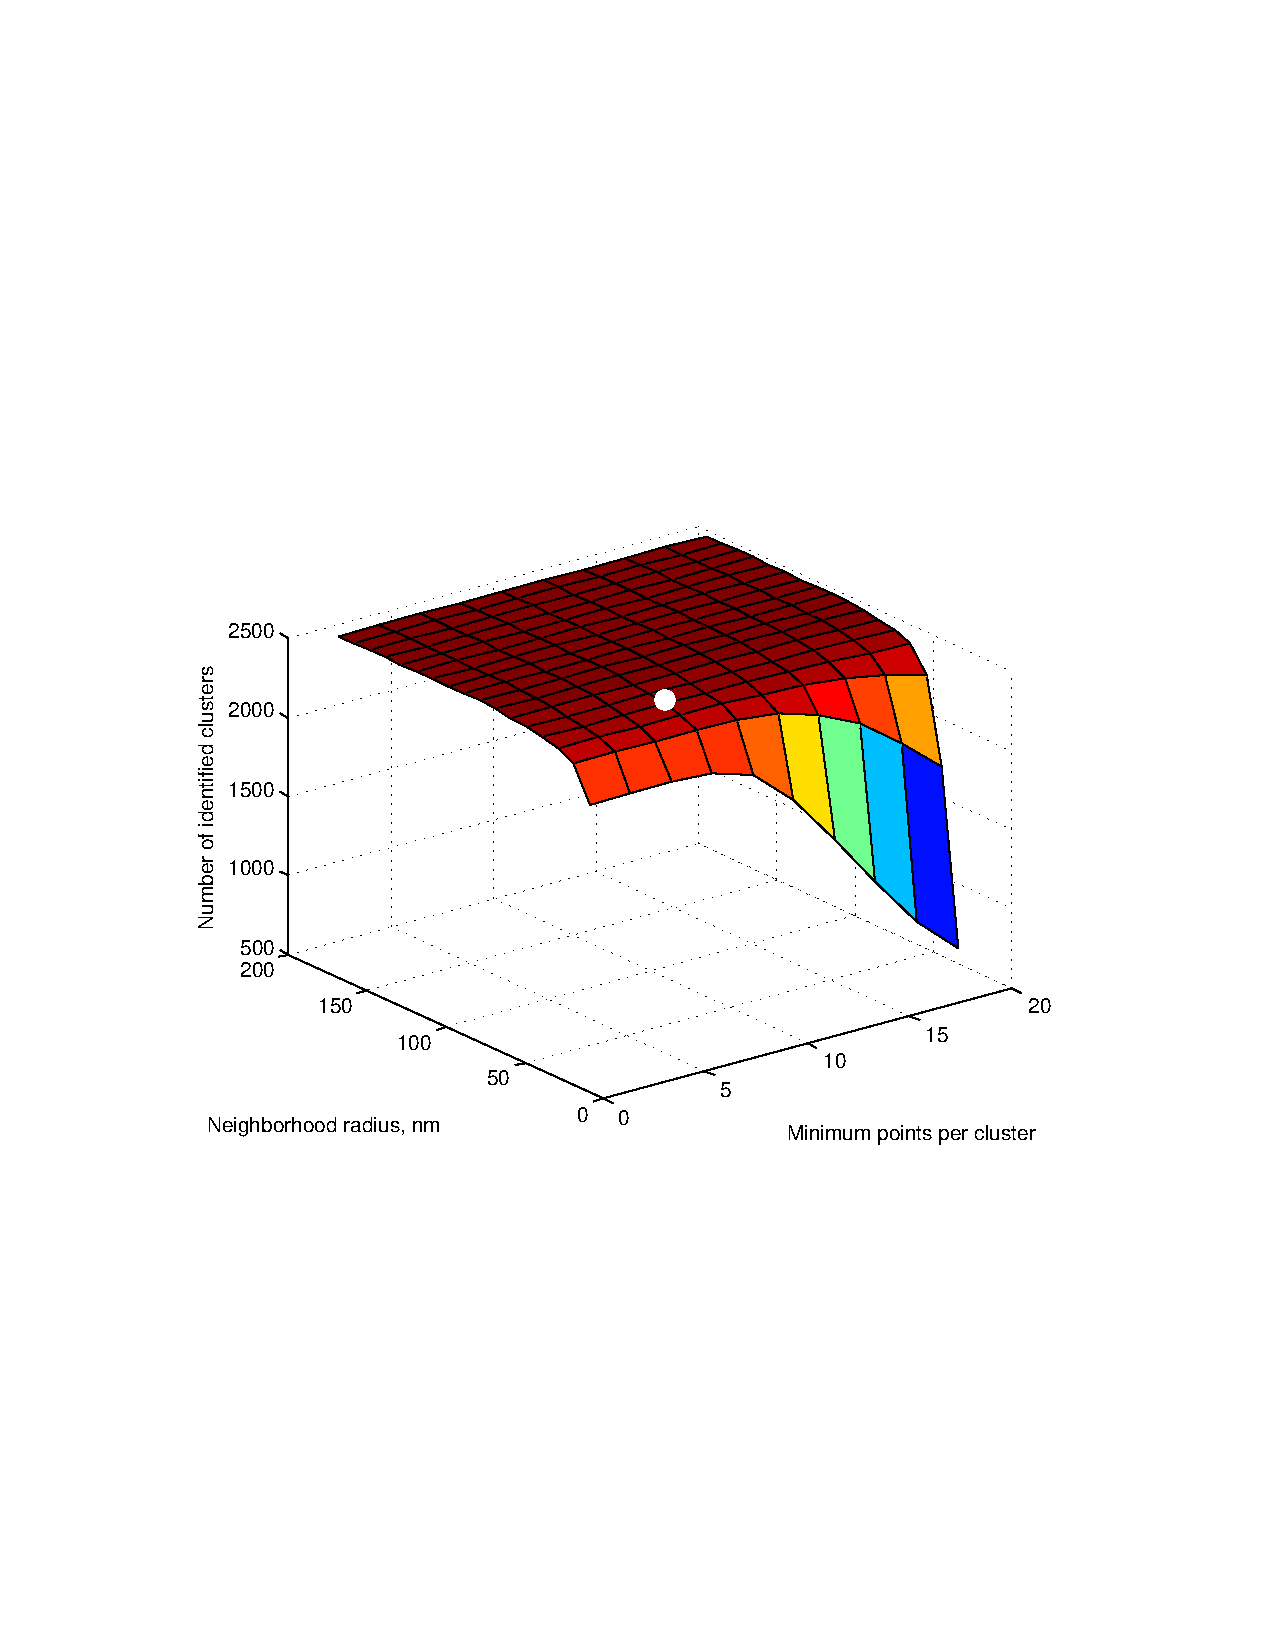
\includegraphics[trim = 0 85mm 0 85mm, clip, scale = 0.6]{fig-dbscan-sweep.pdf}
  \caption{Determining the optimum input parameters for the DBSCAN algorithm. The surface representing the number of identified clusters as a function of the minimum number of localizations per cluster, $k$, and the neighborhood radius, $\epsilon$ is used to find the proper parameter space for isolating single telomeres in the localization datasets. The flat area of the surface where the number of clusters is insensitive to the input parameters indicates a good range of values. The white dot at $\left( k = 8, \epsilon = 65 \right)$ was used for all analyses in this manuscript.}
  \label{fig-dbscan-sweep}
\end{figure}

\subsubsection{Focal volume filtering}
\label{sec-1-2-3}
Axial (z-) coordinates of the localizations were distributed
nonuniformly in the focal volume of the microscope with the
greatest number of localizations identified near the volume's
center transerve plane. Telomeres lying at either extreme of the
axial range of the focal volume may have been truncated due to its
finite extent. Telomeres having a center-of-mass with a
z-coordinate within $100 \; nm$ of the the two extremes were
removed from the analysis to avoid biasing the radius of gyration
distributions. (Note that a shift in the distributions's mean
values of only $\pm 1 \; nm$ was typically observed when filtering
out these extreme telomeres. This indicates that any amount of
bias due to truncated telomeres is very small.)

Clusters that were retained for analysis had axial center-of-mass
coordinates spanning a distance of roughly $600 \; nm$.

\subsubsection{Filtering by number of localizations}
\label{sec-1-2-4}
\label{sec-filter_num_loc}
To ensure sufficient labeling for an accurate determination of the
radius of gyration, telomeres containing fewer than 50
localizations were removed from the analysis. The reason for this
is better explained in Sec. \ref{sec-RgPrecision}. In summary, the
labeling efficiency of a telomere is not 100\%, which means they
are undersampled. Telomere size estimates from fluorophore
localizations are negatively biased by undersampling, and the
magnitude of the bias increases as the number of localizations
decreases.

\subsubsection{Summary of clustering and filtering}
\label{sec-1-2-5}
The grouped, clustered, and filtered localizations were overlayed
with wide field images from the corresponding FOV to ensure that
the clusters corresponded to the individual telomeres and that the
spurious noise in the localization datasets was correctly
eliminated. An example FOV from untransfected Hela L cells with
overlayed and clustered localizations is displayed in
Fig. \ref{fig-widefield-overlay}.

\begin{figure}
  \centering
  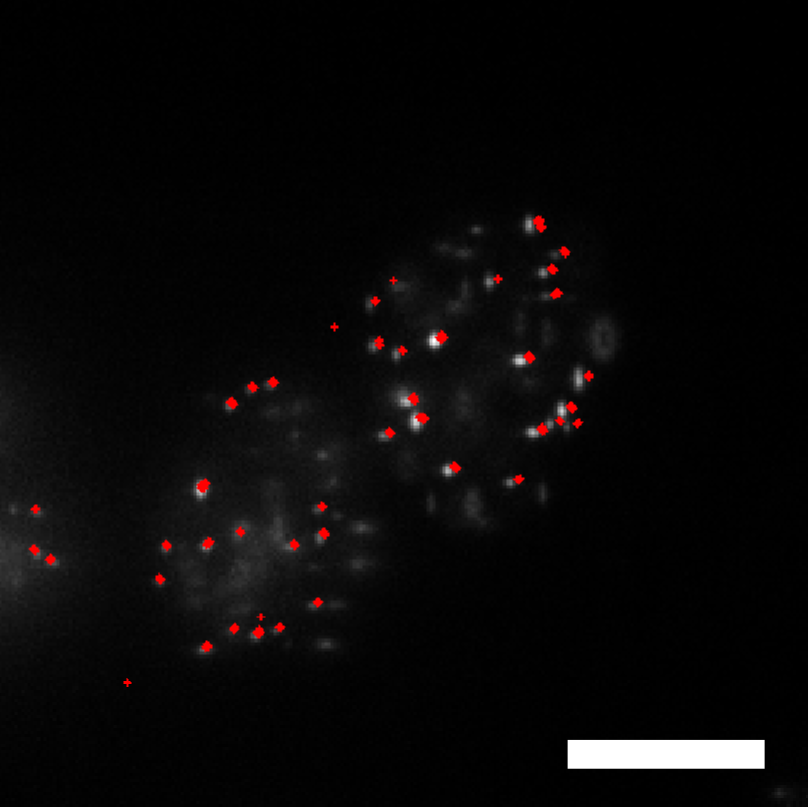
\includegraphics[scale = 0.35]{fig-widefield-overlay.png}
  \caption{A representative widefield image of DNA-FISH labeled telomeres in Hela L cells with localizations belonging to individual telomeres marked in red crosses. Scale bar: $10 \; \mu m$.}
  \label{fig-widefield-overlay}
\end{figure}

\begin{table}[htb]
\centering
\begin{tabular}{|l|p{10cm}|}
\hline
\textbf{Type of clustering/filtering} & \textbf{Parameters used}\\
\hline
Temporal grouping & Keep and group localizations that are on for 10 frames or fewer; Remove localizations on for more than 10 frames\\
\hline
Spatial clustering & Minimum neighborhood number: $k = 8$; neighborhood size: $\epsilon = 65$\\
\hline
Focal volume filtering & Remove clusters with center of mass z-coordinates outside the range $\left[ -300 \, nm, 300 \, nm \right]$\\
\hline
Removing sparse clusters & Clusters with fewer than 50 localizations per cluster are removed from the analysis\\
\hline
\end{tabular}\caption{Summary of filtering and clustering steps performed on the localization datasets.}

\end{table}

\subsection{The radius of gyration as telomere size}
\label{sec-1-3}

\subsubsection{Definition of the radius of gyration}
\label{sec-1-3-1}
The radius of gyration $R_g$ of a single cluster of localizations
is defined by the following expression:

\begin{equation}
\label{eq-rgSquared}
R_g^2 \coloneqq \left[ \frac{1}{n} \sum_{i = 1}^{n} \left( \mathbf{r}_i - \bar{\mathbf{r}} \right)^{\intercal} \left( \mathbf{r}_i - \bar{\mathbf{r}} \right) \right]^{1/2}
\end{equation}

where $n$ is the number of localizations in the cluster,
$\mathbf{r}_i$ is the vector representing the position of the
$i$'th localization, $\bar{\mathbf{r}}$ is the mean position of all
the localizations, and $\intercal$ is the symbol denoting vector
transpose. Eq. \eqref{eq-rgSquared} is equivalent to the
root-mean-square distance of the of localizations from the center
of gravity of the cluster.

The radius of gyration of a linear chain polymer is given by the
same expression as in Eq. \eqref{eq-rgSquared}, except that $n$
becomes the number of Kuhn statistical segments while
$\mathbf{r}_i$ and $\bar{\mathbf{r}}$ represents their individual
positions and mean location, respectively
\cite{flory-statmechchainmolecules-1989}.

In Sec. \ref{sec-RgPrecision} it is empirically demonstrated that
the two different radii of gyration are equivalent to within a
nanometer in the limit that the localization precision goes to
zero and telomeres with fewer than 50 localizations are excluded
from the analysis. In other words, the radius of gyration of the
cluster of localizations is a biased estimator of the radius of
gyration of a telomere's Kuhn statistical segments, and this bias
is less than a nanometer in magnitude. The case of a non-zero
localization precision is treated in Sec. \ref{sec-LocPrecision}.

\subsubsection{Reasons for choosing $R_g$ as a measure of telomere size}
\label{sec-1-3-2}
The radius of gyration was chosen as a measure of telomere size
for the following reasons:
\begin{enumerate}
\item The structure of the data from a STORM experiment suggests a
statistical measure of size. The data consists of a
constellation of localizations in space whose positions are
subject to measurement imprecision and which are randomly
located along the telomere fiber.
\item The end-to-end distance of the telomere fiber could not be
determined. This is because there is no way to differeniate
localizations at the ends of the telomeric region of the
chromatin from localizations found somewhere in the middle.
\item The radius of gyration allows for comparison to polymer models.
\item $R_g$ characterizes a cluster of localizations with a single
number while managing to capture some of the cluster's spatial
non-uniformity.
\end{enumerate}

\subsubsection{Labeling efficiency and precision in $R_g$}
\label{sec-1-3-3}
\label{sec-RgPrecision}
Hela S telomeres were around 10 kbp long, while Hela L telomeres
were about 25 kbp in length. Typically, there were about 100 to 200
localizations identified in each cluster of Hela S and Hela L
telomeres, respectively. Given a DNA-FISH oligonucleotide label
length of 18 bp, this means that the labeling efficiency of
telomeres in this study was only about 0.15 to 0.20.

Because the labeling efficiency is small, a series of simulations
was performed to assess the accuracy and precision in the estimate
of the telomere radius of gyration. 100,000 wormlike chain
conformations were simulated with a packing ratio of $50 \,
    bp/nm$, a persistence length of $50 \, nm$, and a length of $25 \,
    kbp$. Each chain was then downsampled by randomly and uniformly
removing all but a set number of localizations. The mean and
variance of the radius of gyration estimates as a function of the
number of segments preserved in the downsampling are displayed in
Fig. \ref{fig-downsampling}.

\begin{figure}
  \centering
  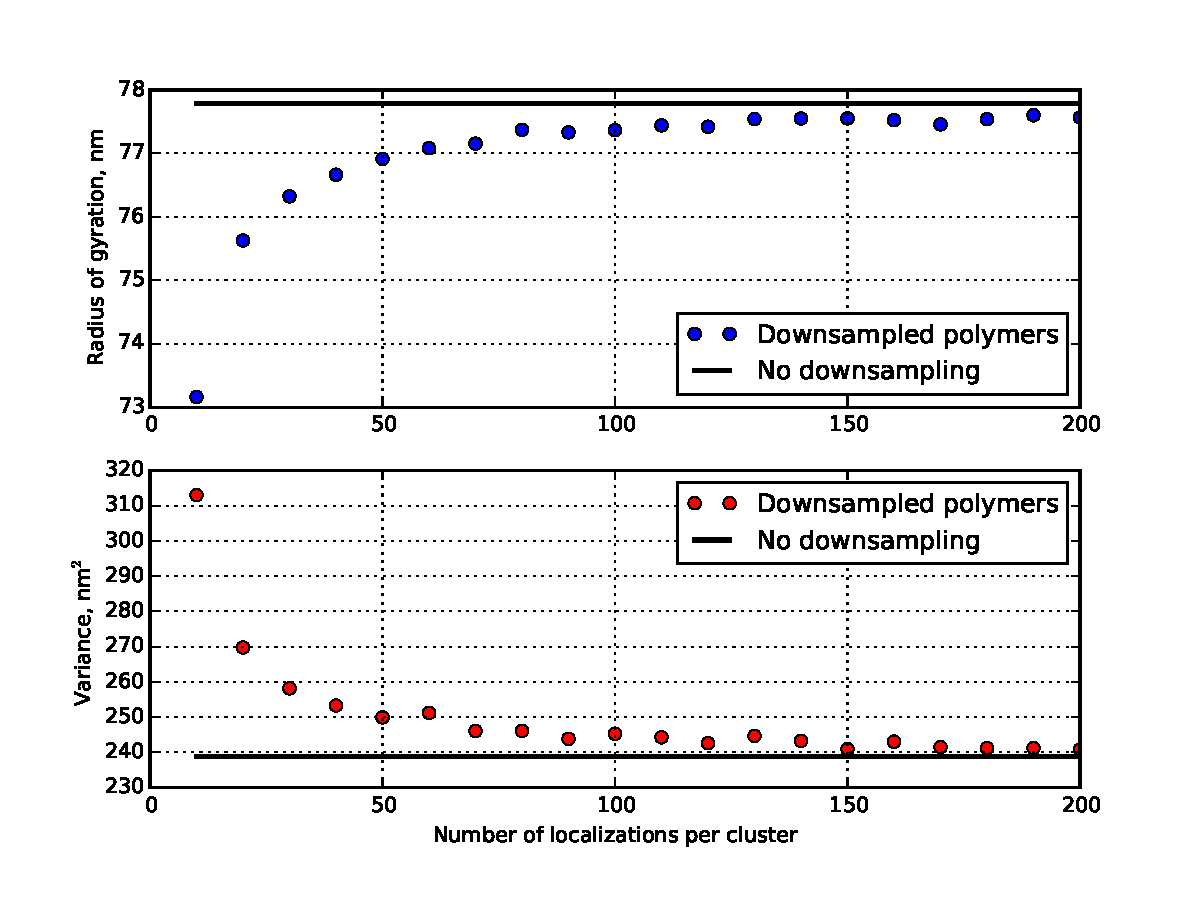
\includegraphics[scale = 0.75]{fig-downsampling_subplots.pdf}
  \caption{The bias in the radius of gyration estimate from a constellation of localizations as a function of the number of localizations. This data was generated by simulating 100,000 different polymer conformations and randomly labeling them with fluorophores. The solid horizontal lines denote the values for the fully-labeled polymer. The polymers were generated from an ensemble with a packing ratio of $50 \, bp/nm$, a persistence length of $\ell_p = 50 \, nm$, and a length of $25 \, kbp$.}
  \label{fig-downsampling}
\end{figure}

The results of the simulations presented in
Fig. \ref{fig-downsampling} show that, for the given set of
simulated polymer parameters, telomeres with fifty or more
localizations will have, on the average, $R_g$ values within one
nanometer and a variance in $R_g$ that is less than 5\% of the
real population of telomeres.

In general, the bias should be even less for shorter or more
compact telomeres because they would not require as many labels to
accurately determine their real radius of gyration. For longer or
less compact telomeres, the bias will be worse. The lower cutoff
for filtering clusters based on their number of localizations was
set to 50 in all analyses as discussed in
Sec. \ref{sec-filter_num_loc}. This was chosen as a compromise
between accurately determing the radius of gyration of a telomere
based on a constellation of localizations and excluding very small
and sparsely labeled telomeres in the size distributions.

Another source of error, namely the precision in the location of a
fluorophore, will add an additional bias to the $R_g$
estimate. This bias is taken into account in the maximum
likelihood estimates of the polymer parameters in
Sec. \ref{sec-MLE}.

\section{Polymer modeling of STORM datasets}
\label{sec-2}

\subsection{The wormlike chain model}
\label{sec-2-1}
The wormlike chain (WLC) was chosen as the polymer model in this
work because it has been successfully applied in studies of
chromatin conformation at similar genomic length scales as those of
Hela telomeres \cite{bystricky-pnas-2004, huet-2014} and because it
can be easily compared to other models of chromatin packaging, such
as the 10 nm and 30 nm fibers.

The WLC, also known as a Kratky-Porod chain
\cite{kratkyporod-1949}, describes an equilibrium ensemble of
polymer conformations.  In the simplest WLC model, the polymer is
treated as a continuous, semiflexible, and homogeneous rod whose
conformation is deformed by thermal interactions with its solvent
environment. The simple WLC model has a negligible thickness and a
length $L_c$, otherwise known as the contour length. The
flexibility of the rod is described by its persistence length
$\ell_p$. Intuitively, the persistence length is the average length
over which the polymer remains approximately straight. Polymers
with a longer persistence length will be more rigid than shorter
ones.

Mathematically, the persistence length is the characteristic length
describing the exponential decay of the tanget-tanget correlation
function of an infinitely long WLC
\cite{phillips-pbotc-2009, schellman-biopolymers-1974},

\begin{equation}
  \label{eq-tantancorr}
  \left< \mathbf{t} \left( s \right) \cdot \mathbf{t} \left( 0 \right) \right> \sim \exp \left( -s / \ell_p \right)
\end{equation}

where $\mathbf{t} \left( s \right)$ is the unit vector tangent to
the polymer at the one-dimensional coordinate $s$ along the
polymer. For distances $s$ much greater than $\ell_p$, Eq.
\eqref{eq-tantancorr} shows that there will be no correlation in
the direction that the tangent vectors point.

The mean-square radius of gyration of an ensemble of WLC's with the
same contour length and persistence length is \cite{nakamura-2008}

\begin{equation}
  \label{eq-meanWLCRg}
  \left< R_{g}^2 \right> = \frac{2 L_{c} \ell_{p}}{6} - \ell_{p}^2 + \left( \frac{2 \ell_p^3}{L_c^2} \right) \left[ L_c - \ell_p \left( 1 - e^{-L_c/\ell_p} \right) \right]
\end{equation}

In the limit that the contour length $L_c$ becomes much larger than
the persistence length $\ell_p$, Eq. \eqref{eq-meanWLCRg} tends to
$2 L_c \ell_{p}/6$, which is equivalent to the expression for the
mean-square radius of gyration of the freely-jointed chain
(sometimes known as the Gaussian chain) \cite{phillips-pbotc-2009}.

\subsubsection{The second moment of the WLC bending angle distribution}
\label{sec-2-1-1}

Linear, semiflexible polymers are composed of small molecules and
are thus subject to agitation by the random collisions with
solvent molecules in their environment. These collisions cause the
polymer to adopt one of many random configurations at any given
moment in time. According to Boltzmann's statistics, the
probability that a semiflexible polymer in thermodynamic
equilibrium will be found in one of any of its possible
conformations is proportional to the Boltzmann factor

\begin{equation}
  \label{eq-boltzmann}
  P \left( U \right) \sim \exp \left( -\frac{U}{k_B T}\right)
\end{equation}

where $P \left( U \right)$ represents of the probability of
observing a polymer conformation with associated free energy $U$,
$k_B$ is Boltzmann's constant and $T$ is the absolute temperature
of the system. The fact that it takes energy to bend the polymer
into a particular conformation reflects the ``semiflexible''
qualities of the polymer.

The energy $U$ required from the environment to achieve a given
conformation can be determined by dividing the polymer into many
short sections such that it can be reprensented as the summation
of the bending energies of many small circular arcs
\cite{phillips-pbotc-2009}. The energy required to bend a rod
through an angle $\theta$ with Young's modulus $E$ and moment of
inertia $I$ is

\begin{equation}
\label{eq-bending-energy}
  U = \frac{EI}{2s}\theta^{2}
\end{equation}

Now consider a continuously bending WLC in three dimesions. If the
initial unit tangent vector at its origin points in the
z-direction, then the dot product with the unit tangent vector at
any other position $s$ along the chain is just the cosine of the
angle between the tangent vectors. The tangent-tangent correlation
function in Eq. \eqref{eq-tantancorr} is then

\begin{align}
  \langle \mathbf{t} \left( s \right) \cdot \mathbf{t} \left( 0 \right) \rangle &= \langle \cos \theta\rangle \\
  &\approx \left< 1 - \frac{\theta^2 \left( s\right) }{2} \right> \label{eq-cosineseries}
\end{align}

where all but the first two terms in the power series expansion
for the cosine have been dropped in the last line. The
thermodynamic average of $\left< \theta^2 \left( s \right)
    \right>$ can be determined by using Eq. \eqref{eq-bending-energy}
and integrating $\theta^2 \left( s \right) \exp \left( -U /
    k_{B}T\right)$ over a full $4 \pi$ solid angle in three dimensions
and then dividing by the partition function. This calculation is
carried out in Ref. \cite{phillips-pbotc-2009}. The result is

\begin{align}
  \left< \theta^2 \left( s \right) \right> &= \frac{2 k_{B} Ts}{EI} \\
  &= \frac{2s}{\ell_p} \label{eq-thetaM2}
\end{align}

where the definition of the persistence length $\ell_p \coloneqq
    EI/k_{B}T$ is used in Eq. \eqref{eq-thetaM2}.

Eq. \eqref{eq-thetaM2} is significant because it specifies the
second moment of a probability distribution for the bending angle
as a function of the distance along the WLC and its persistence
length. This moment can be used when generating random numbers
that simulate the conformation of a polymer, as described in the
next section.

\subsection{Wormlike chain simulation}
\label{sec-2-2}
A continuous WLC may be simulated by approximating the chain
contour as a series of discrete line segments of equal length with
a random angle between the line segments. According to
Eq. \eqref{eq-cosineseries} and Eq. \eqref{eq-thetaM2}, the first
moment of the probability distribution function that describes the
angle between any two line segments in a WLC is zero and the second
moment is $2s/\ell_p$, where $s$ is now considered to be the length
of a line segment. Since higher order moments were truncated in the
power series expansion in Eq. \eqref{eq-cosineseries}, we can
approximate a WLC by drawing a series of line segments with angles
between the line segments determined by random numbers generated
from a zero-mean Gaussian distribution having a variance given by
Eq. \eqref{eq-thetaM2}.

This approach was used in Ref. \cite{rivetti-jmolbiol-1996} to
simulate WLC's in two dimensions. In three dimensions, the line
segments are no longer confined to a plane, which means the
chain-generating algorithm must allow for an additional random
rotation.

The algorithm for generating a three dimensional WLC based on
these probability distribution functions is as follows:

\begin{algorithm}
  \caption{Generating 3D wormlike chains}
  \label{alg-3dWLC}
  \begin{algorithmic}[1]
    \Require{A persistence length $\ell_p$ and a number of segments $N$}
    \Statex
    \State $i\gets 1$
    \State $\mathbf{r}_1\gets \hat{x}$ \Comment{$\mathbf{r}_{1}$ is a unit vector in the x-direction}
    \While{$i \leq N$}
      \State $\theta\gets \text{Gaussian random number with variance equal to } 2/\ell_{p}$
      \State $\mathbf{a}\gets \text{uniformly and randomly oriented unit vector}$
      \Statex
      \While{$\mathbf{r}_i \times \mathbf{a} = 0$}
        \State $\mathbf{a}\gets \text{uniformly and randomly oriented unit vector}$
      \EndWhile
    \Statex
    \State $\mathbf{d}\gets \left( \sin \theta \right) \frac{\mathbf{r}_i \times \mathbf{a}}{\lVert \mathbf{r}_i \times \mathbf{a} \rVert}$ \Comment{$\mathbf{d}$ is perpendicular to $\mathbf{r}_i$}
    \State $\mathbf{r}_{i+1}\gets \mathbf{r}_i \left( \cos \theta \right) + \mathbf{d}$
    \State $i\gets i + 1$
    \EndWhile
    \Statex 
    \State $\text{path} \gets \mathbf{cumsum} \{ \mathbf{r}_i \}$ \Comment{$\mathbf{cumsum}$ is the cumulative summation of a set}
  \end{algorithmic}
\end{algorithm}

This algorithm generates the WLC by generating a random walk on the
surface of the unit sphere. Each point on the walk is represented
by a vector $\mathbf{r}_i$ point from the origin to the
surface. The polymer is created in the end by cumulatively summing
all the vectors in the ordered set $\{\mathbf{r}_i\}$ that form the
random walk. The $\times$ operator denotes the vector cross product
and $\lVert \cdots \rVert$ denotes the Euclidean norm of a vector.

\subsubsection{Accuracy of the simulation}
\label{sec-2-2-1}

\subsection{Generating STORM datasets from wormlike chain ensembles}
\label{sec-2-3}

\subsubsection{Accounting for localization precision}
\label{sec-2-3-1}
\label{sec-LocPrecision}

\section{Maximum likelihood estimation of polymer parameters}
\label{sec-3}
\label{sec-MLE}
\section{Abbreviations}
\label{sec-4}
\begin{description}
\item[{DBSCAN}] Density-based spatial clustering of applications with
noise
\item[{FOV}] Field of view
\item[{PSF}] Point spread function
\item[{WLC}] Wormlike chain
\end{description}

\printbibliography
% Emacs 24.4.50.1 (Org mode 8.2.6)
\end{document}
